\title{CS313 : DataBases and Information Systems Lab \\
    \vspace{0.6cm}
    Lab Assignment 3
} % You may change the title if you want.
% \subtitle{Hello}
\author{Sourabh Bhosale \\ 200010004}

\date{\today}

\documentclass[12pt]{article}
\usepackage{fullpage}
\usepackage{enumitem}
\usepackage{amsmath,mathtools}
\usepackage{amssymb}
\usepackage[super]{nth}
\usepackage{textcomp}
\usepackage{hyperref}
\usepackage{multicol}
\usepackage{multirow}
\usepackage{minted}
% \usepackage{fontspec}
% \usepackage[showframe]{geometry}

% \usepackage[default]{sourcesanspro}
% \usepackage[T1]{fontenc}

% \usepackage[sfdefault]{noto}
% \usepackage[T1]{fontenc}

\usepackage[default,oldstyle,scale=0.95]{opensans} %% Alternatively
%% use the option 'defaultsans' instead of 'default' to replace the
%% sans serif font only.
\usepackage[T1]{fontenc}

% \setmainfont{Roboto}
\usepackage{titling}
\hypersetup{
    colorlinks=true,
    linkcolor=blue,
    filecolor=magenta,      
    urlcolor=cyan,
}

\renewcommand\maketitlehooka{\null\mbox{}\vfill}
\renewcommand\maketitlehookd{\vfill\null}

\begin{document}


\begin{titlingpage}
\maketitle
\end{titlingpage}

\newpage
%---------------------------------------------------------------------

% \begin{tiny}
\section{Creating User and Database called lab3}

\subsection{Query}
\fbox{ 
    \begin{minipage}{40em}
    \inputminted{mysql}{src/question1.sql}
    \end{minipage}
}

\subsection{Result}
\begin{figure}[hbt]
    \centering
    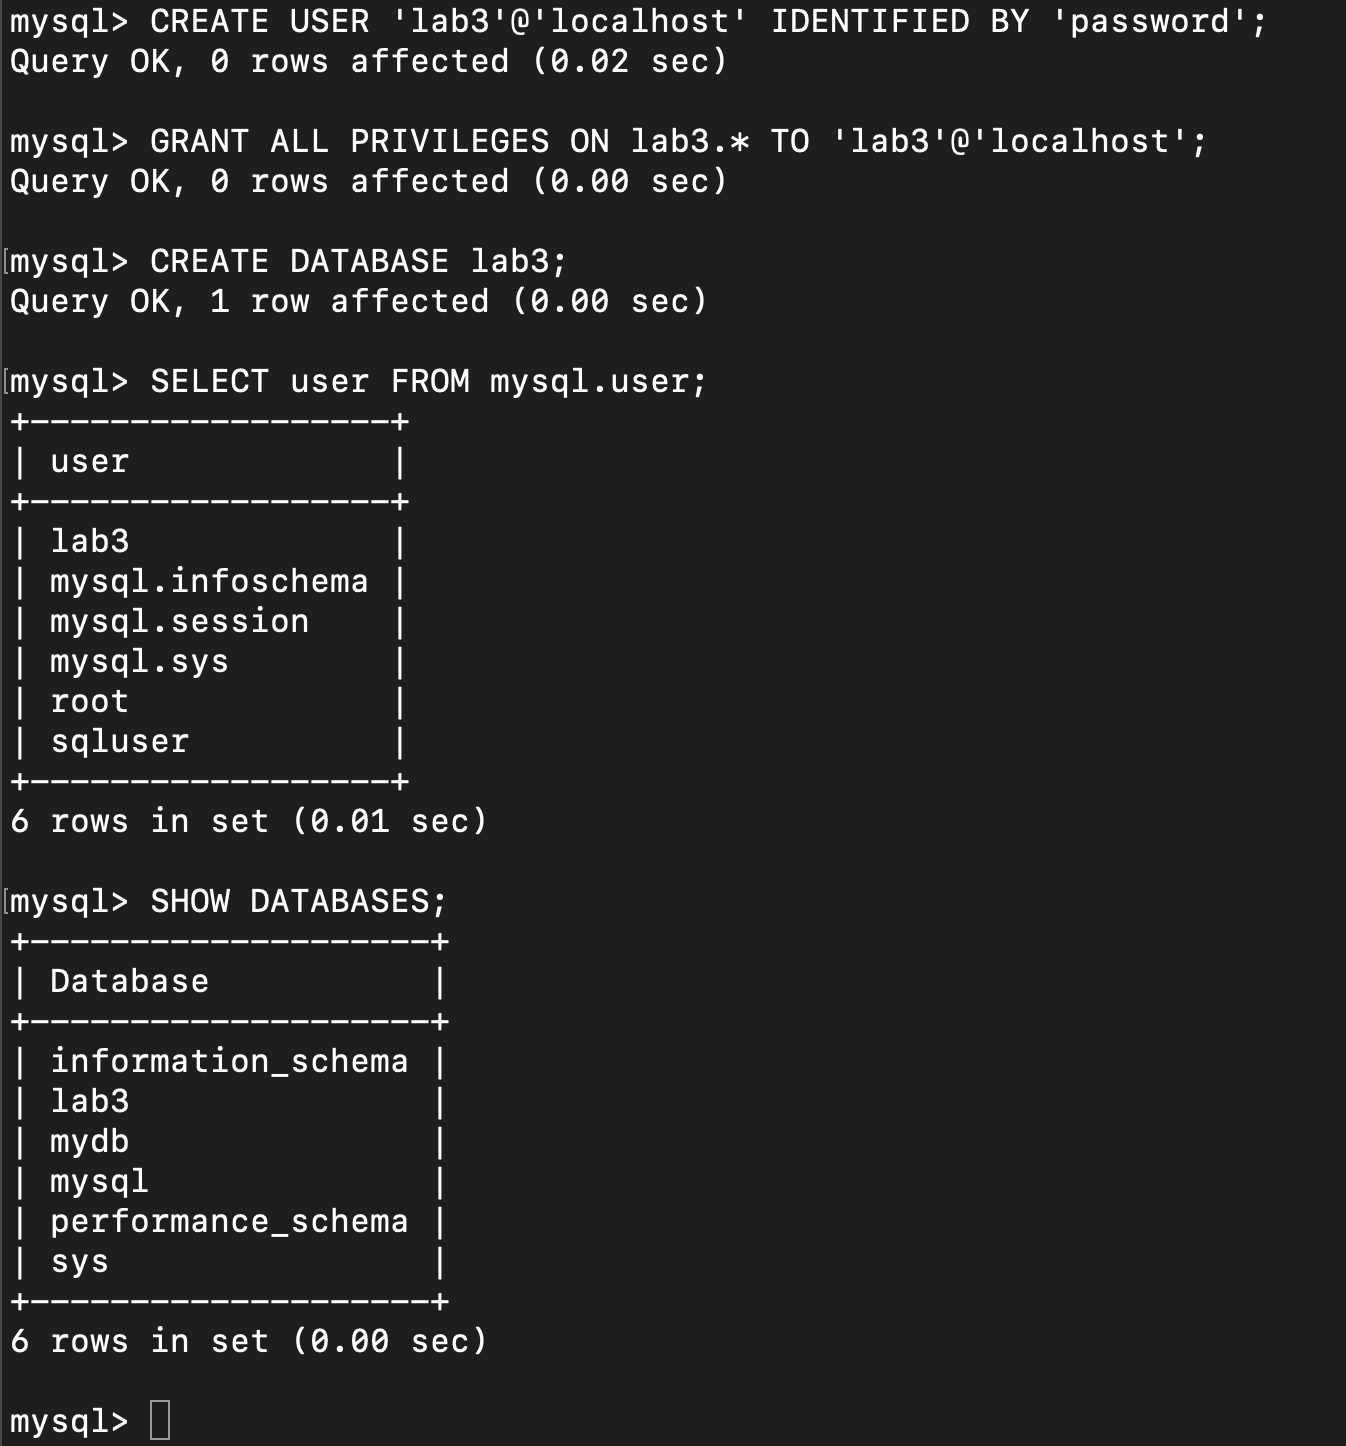
\includegraphics[scale=0.55]{screenshots/1.png}
    \label{fig:my_label1}
\end{figure}

\newpage
%---------------------------------------------------------------------

\section{Creating the tables: part, supplier, shipment}

\subsection{Query}
\fbox{ 
    \begin{minipage}{40em}
    \inputminted{mysql}{src/question2.sql}
    \end{minipage}
}
\newpage
\subsection{Result}
\begin{figure}[!hbt]
    \centering
    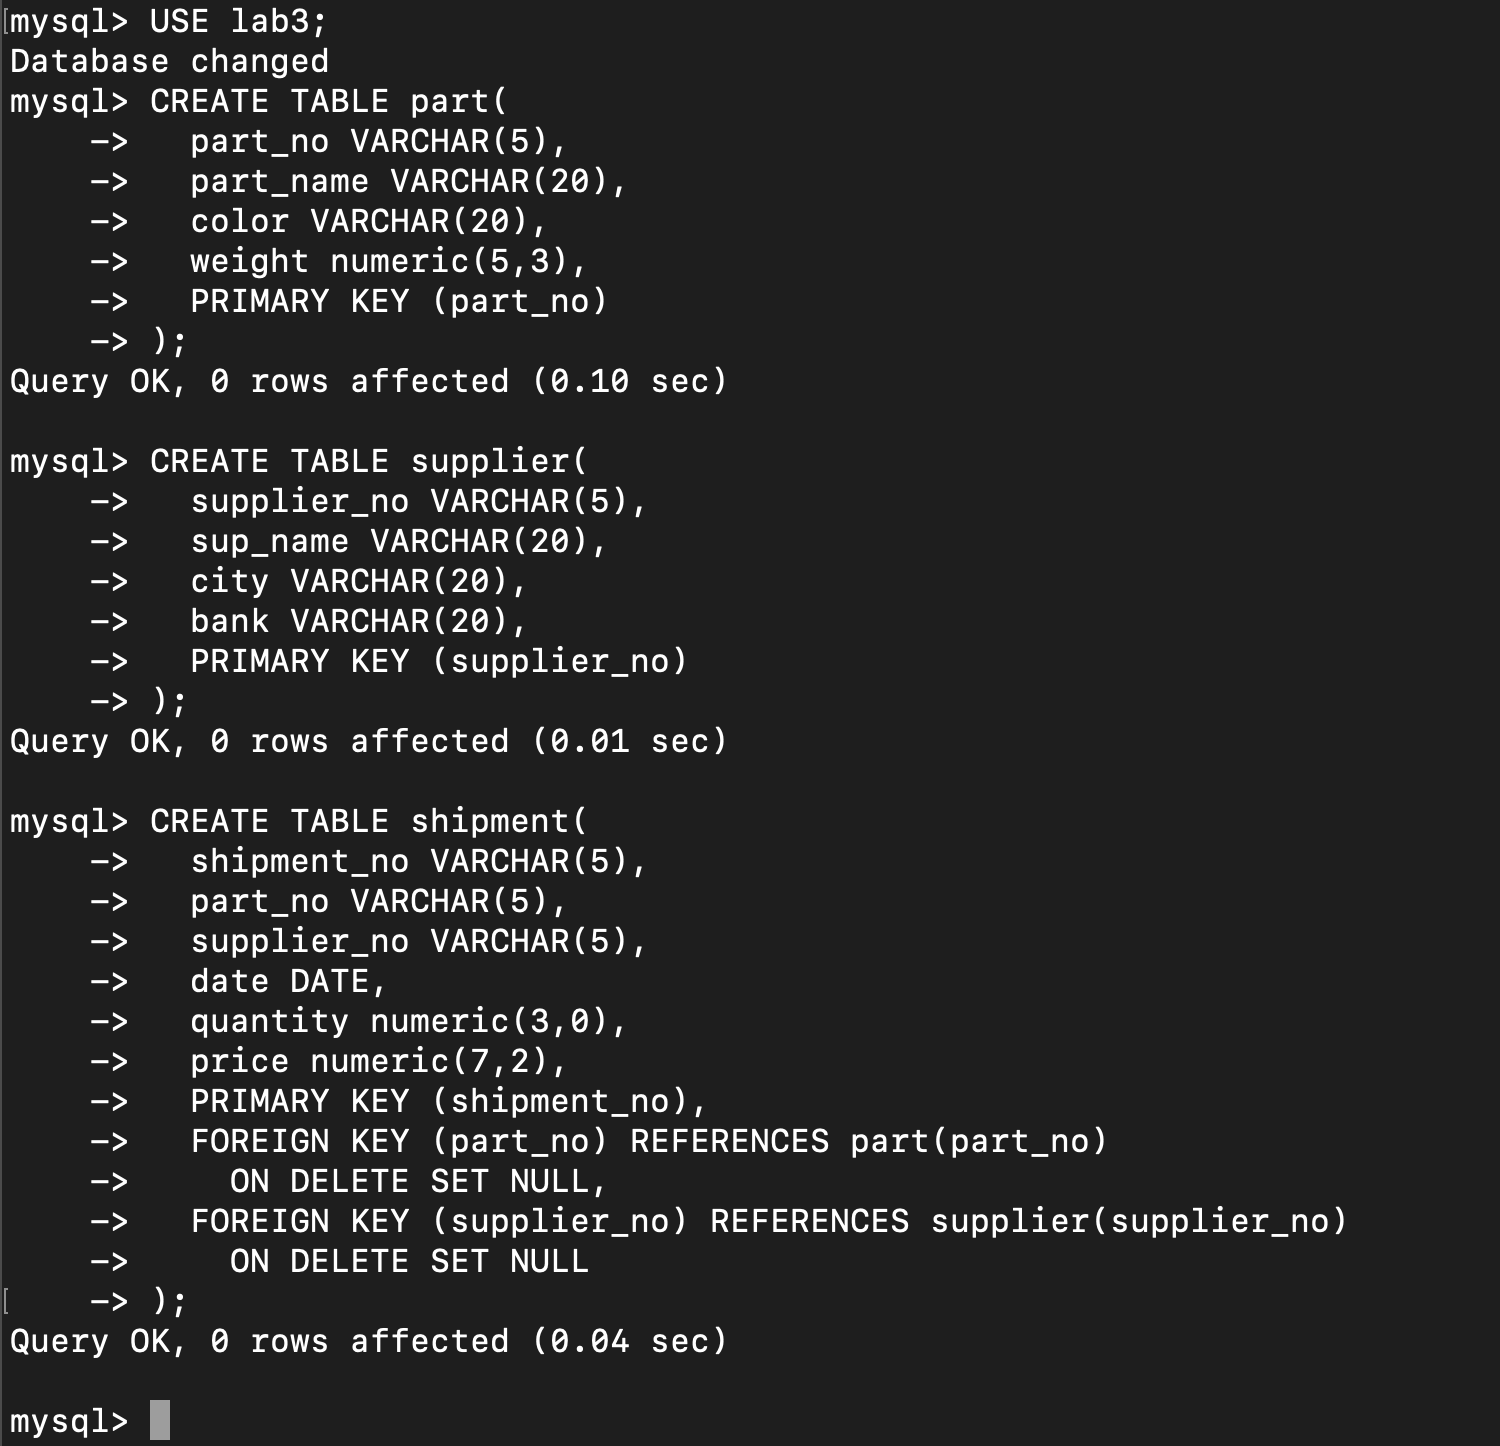
\includegraphics[scale=0.65]{screenshots/2.png}
    \label{fig:my_label1}
\end{figure}
\newpage

%---------------------------------------------------------------------

\section{Adding one tuple in each table using the mysql \textit{insert} statement}

\subsection{Query}
\fbox{ 
    \begin{minipage}{40em}
    \inputminted{mysql}{src/question3.sql}
    \end{minipage}
}

\subsection{Result}
\begin{figure}[!hbt]
    \centering
    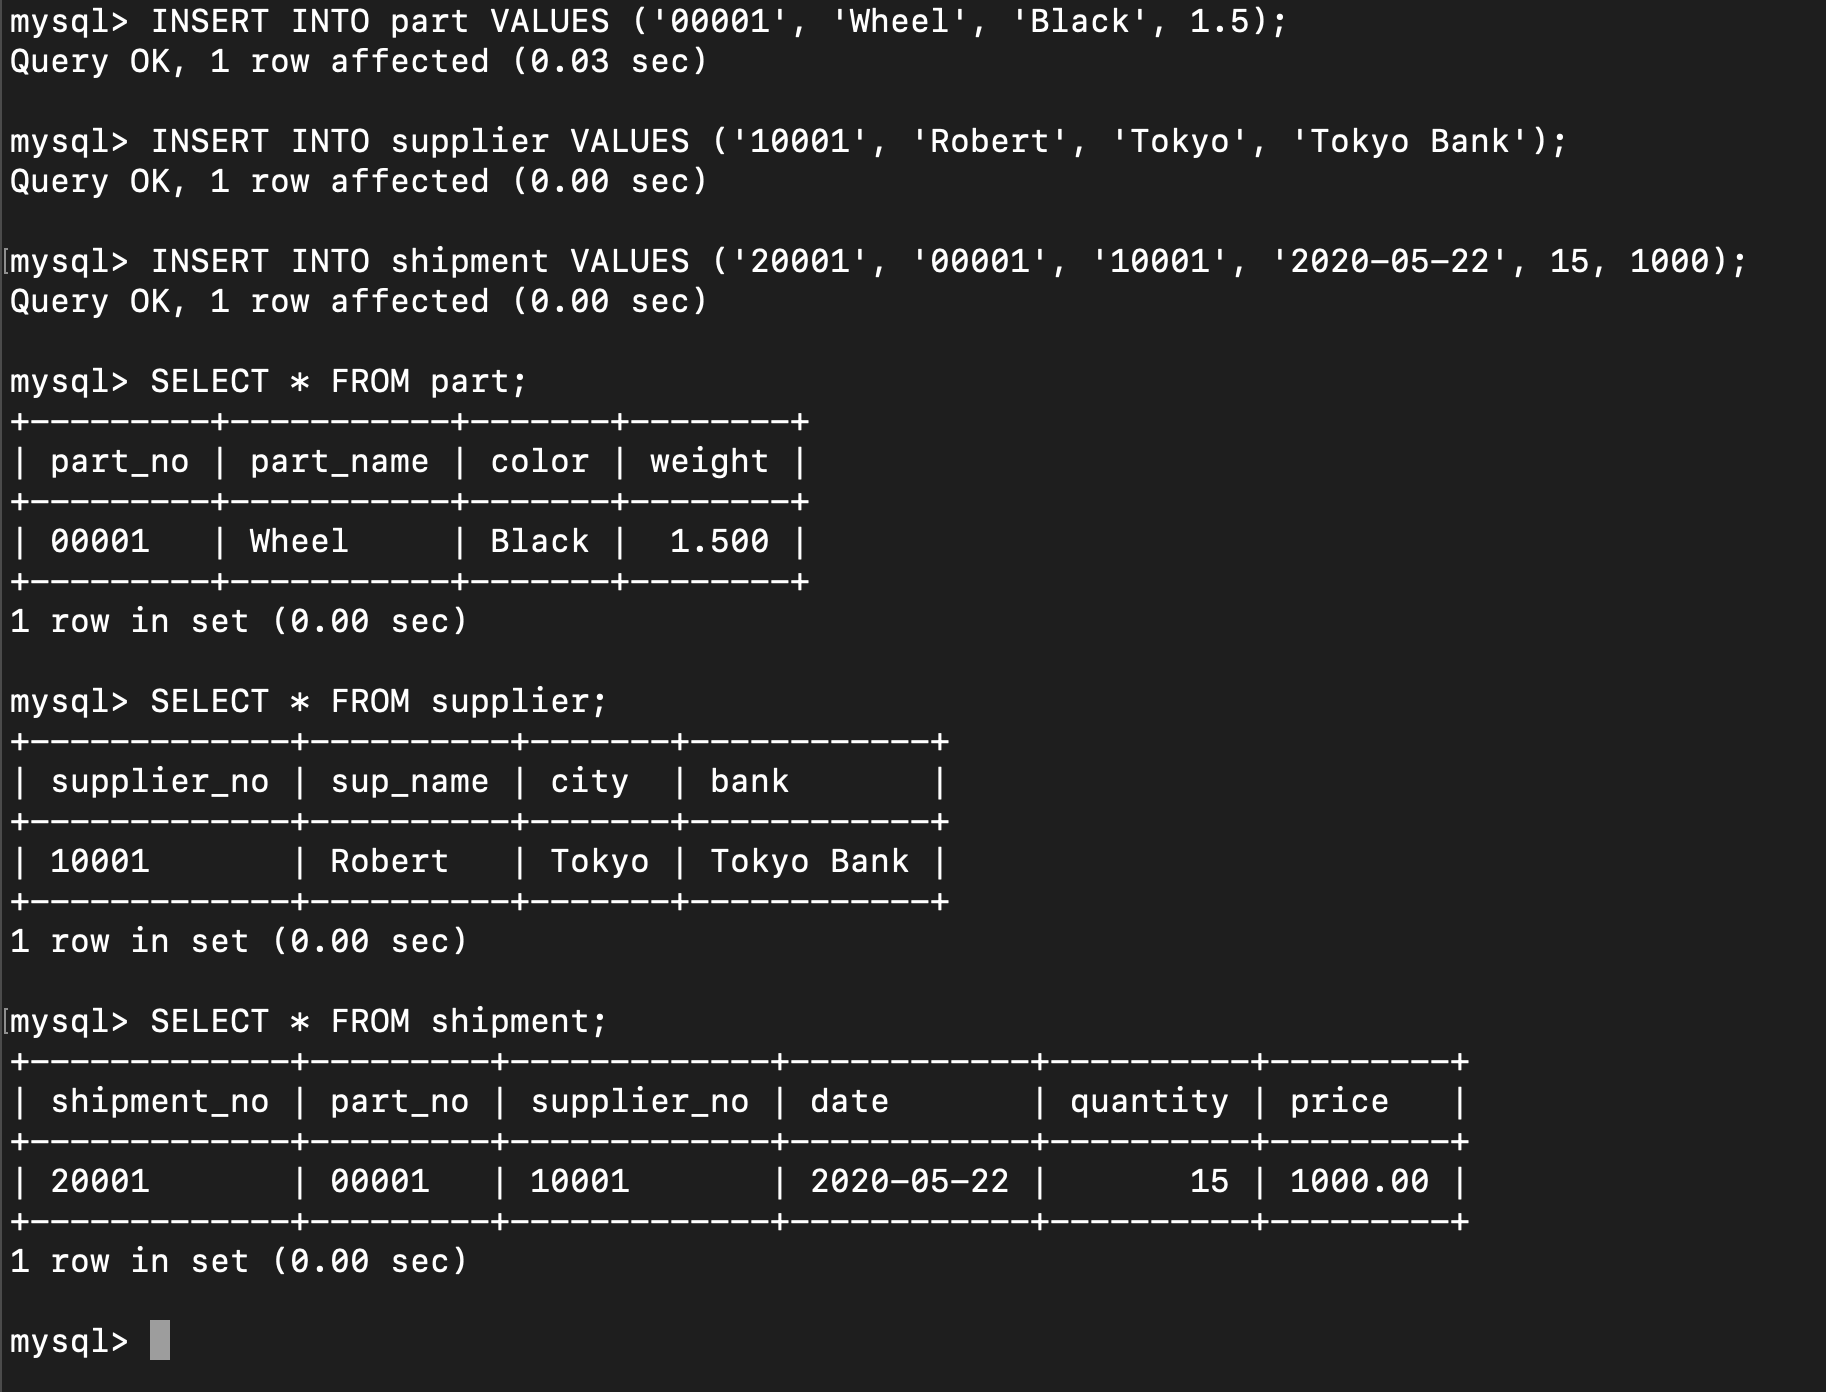
\includegraphics[scale=0.55]{screenshots/3.png}
    \label{fig:my_label1}
\end{figure}

\newpage
%--------------------------------------------------------------

\section{Inserting more data in the tables}

\subsection{Query}
\fbox{ 
    \begin{minipage}{40em}
    \inputminted{mysql}{src/question4.sql}
    \end{minipage}
}
\newpage

\subsection{Results}
\begin{figure}[!hbt]
    \centering
    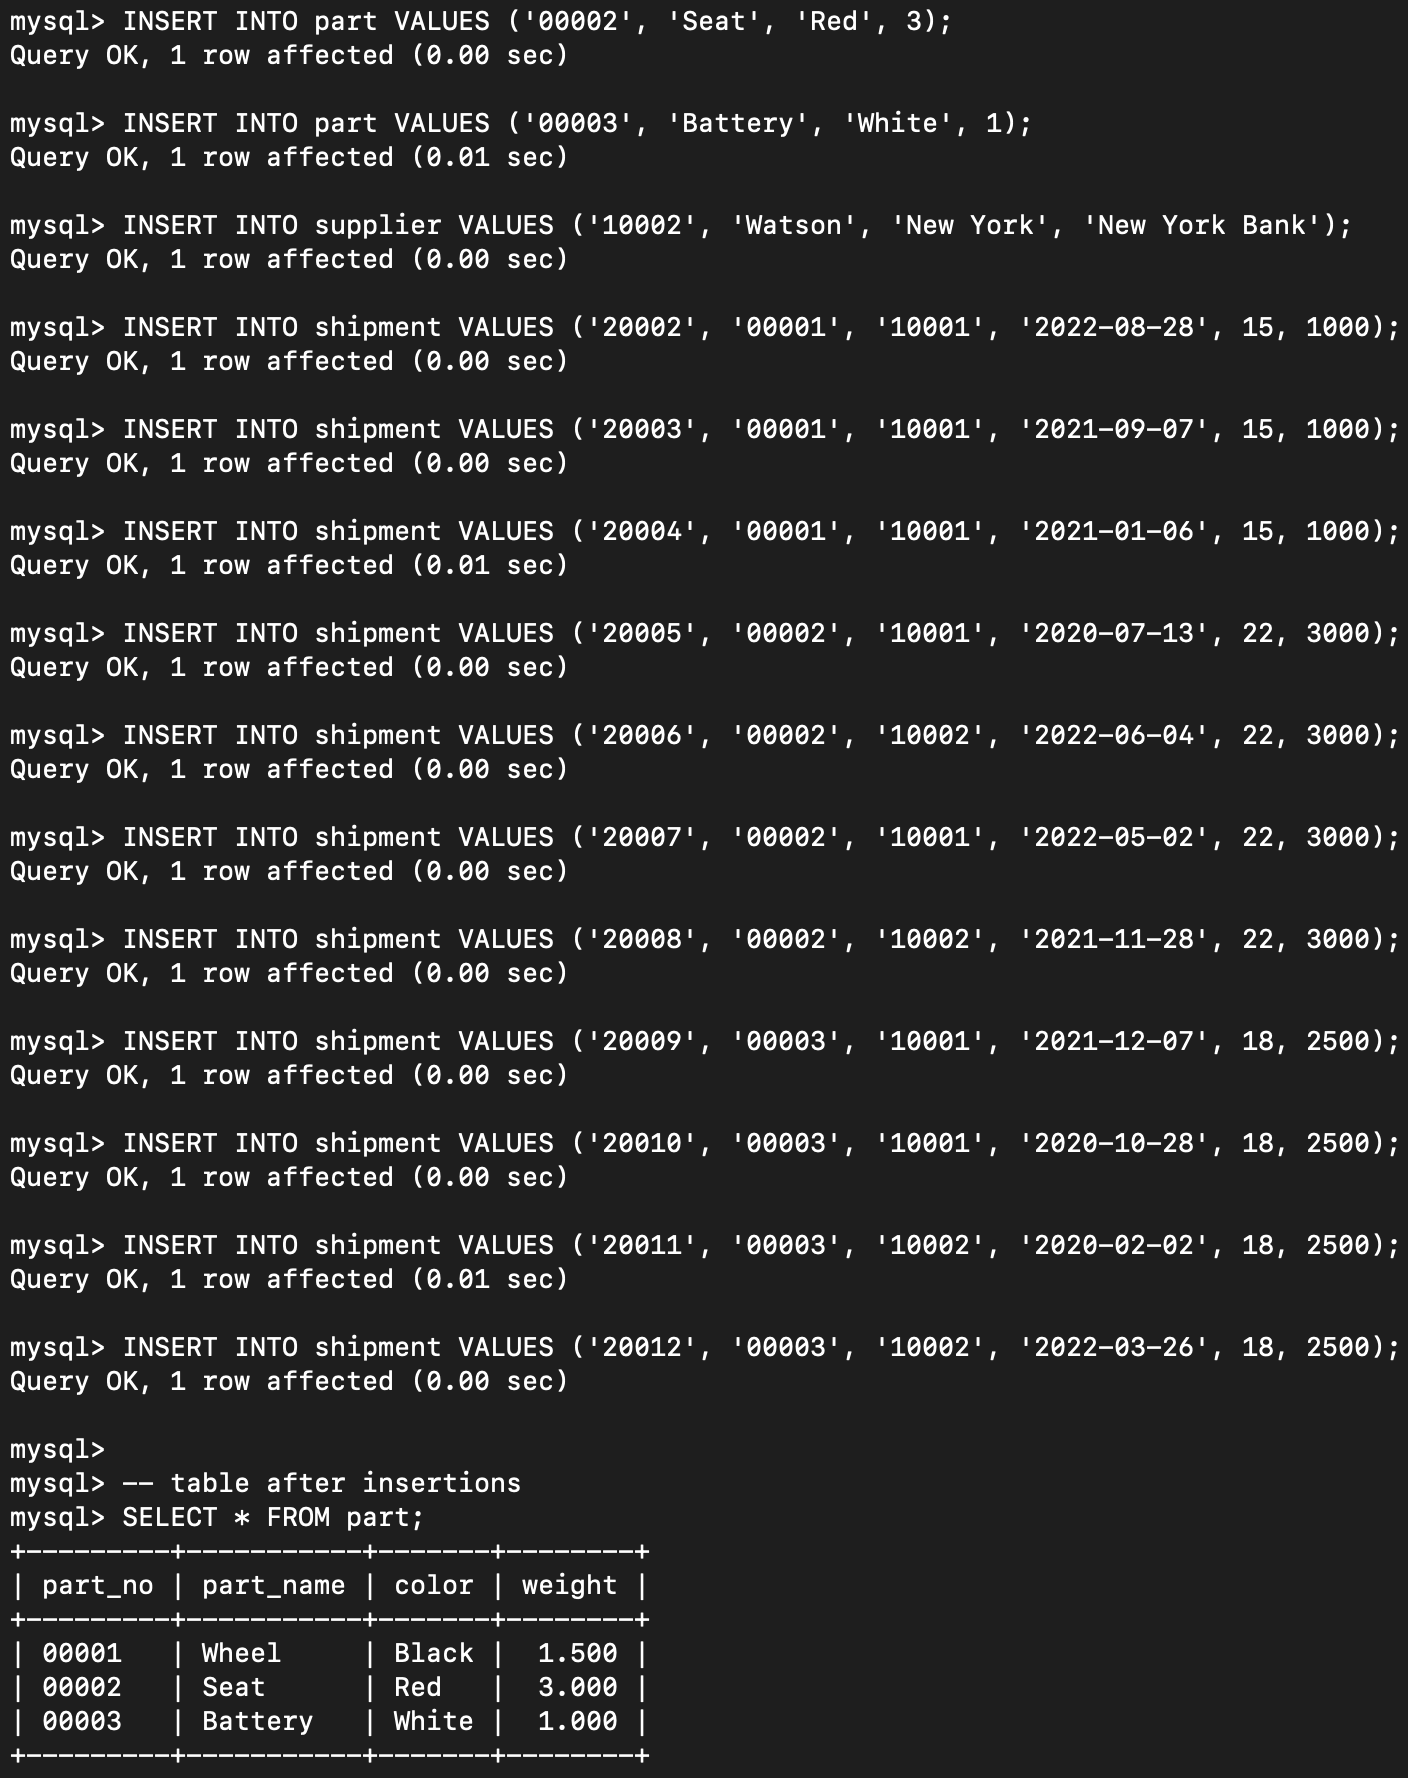
\includegraphics[scale=0.65]{screenshots/4a.png}
    \label{fig:my_label1}
\end{figure}
\newpage
\begin{figure}[!hbt]
    \centering
    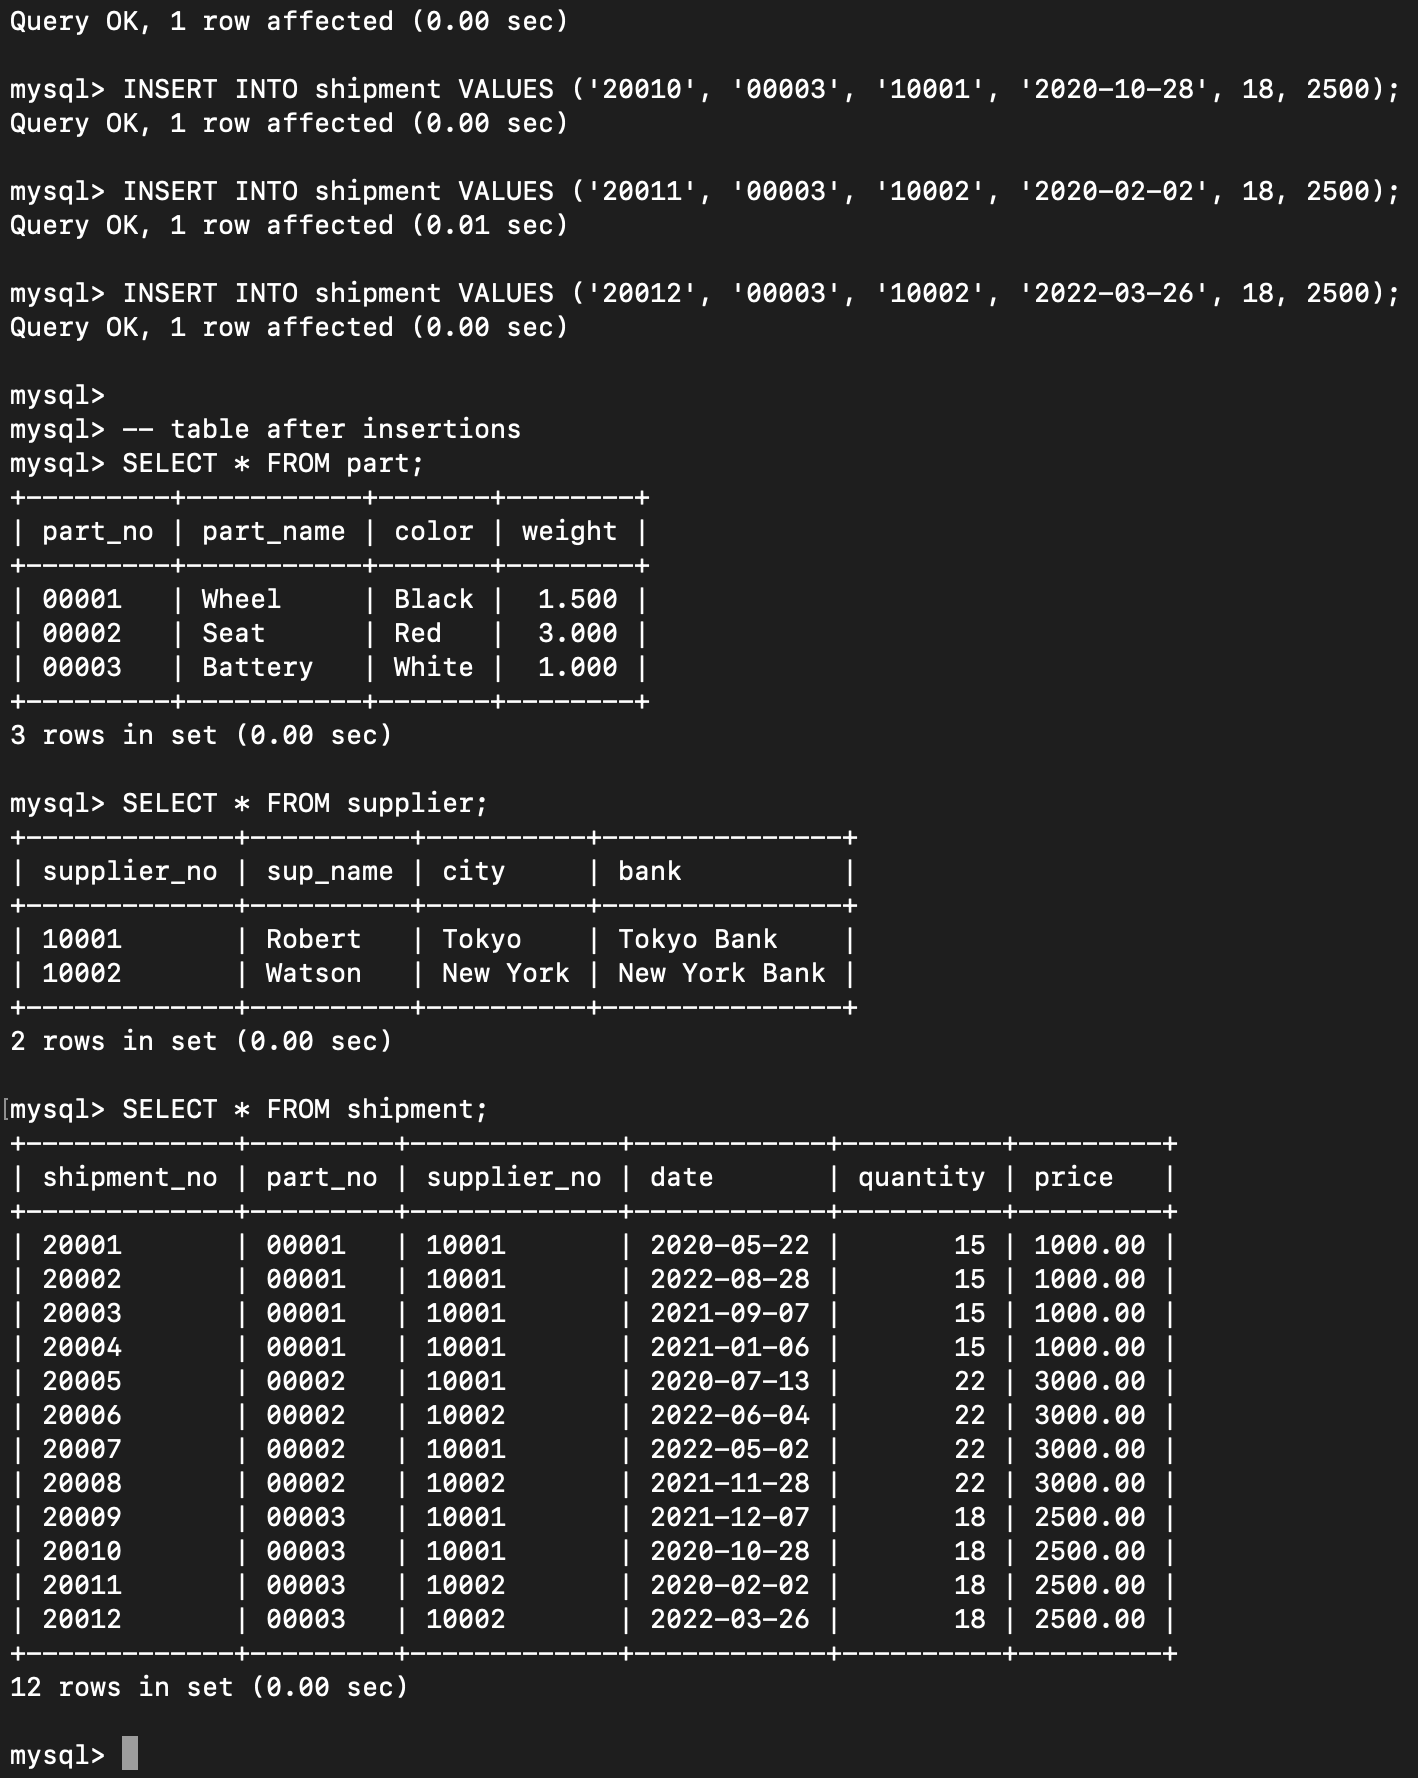
\includegraphics[scale=0.65]{screenshots/4b.png}
    \label{fig:my_label1}
\end{figure}
\newpage
%--------------------------------------------------------------

\section{Additional queries}

\subsection{Suppliers who have supplied red parts}

\subsubsection{Query}
\fbox{ \begin{minipage}{40em}
\inputminted{mysql}{src/question5a.sql}
\end{minipage}
}

\subsubsection{Result}
\begin{figure}[!hbt]
    \centering
    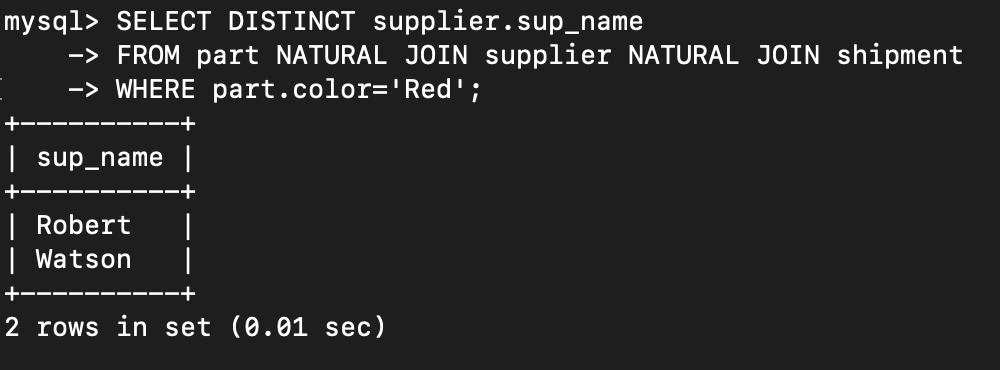
\includegraphics[scale=1.0]{screenshots/5a.png}
    \label{fig:my_label1}
\end{figure}

\subsection{Total cost of shipments for all suppliers}

\subsubsection{Query}
\fbox{ \begin{minipage}{40em}
\inputminted{mysql}{src/question5b.sql}
\end{minipage}
}
\newpage
\subsubsection{Result}
\begin{figure}[!hbt]
    \centering
    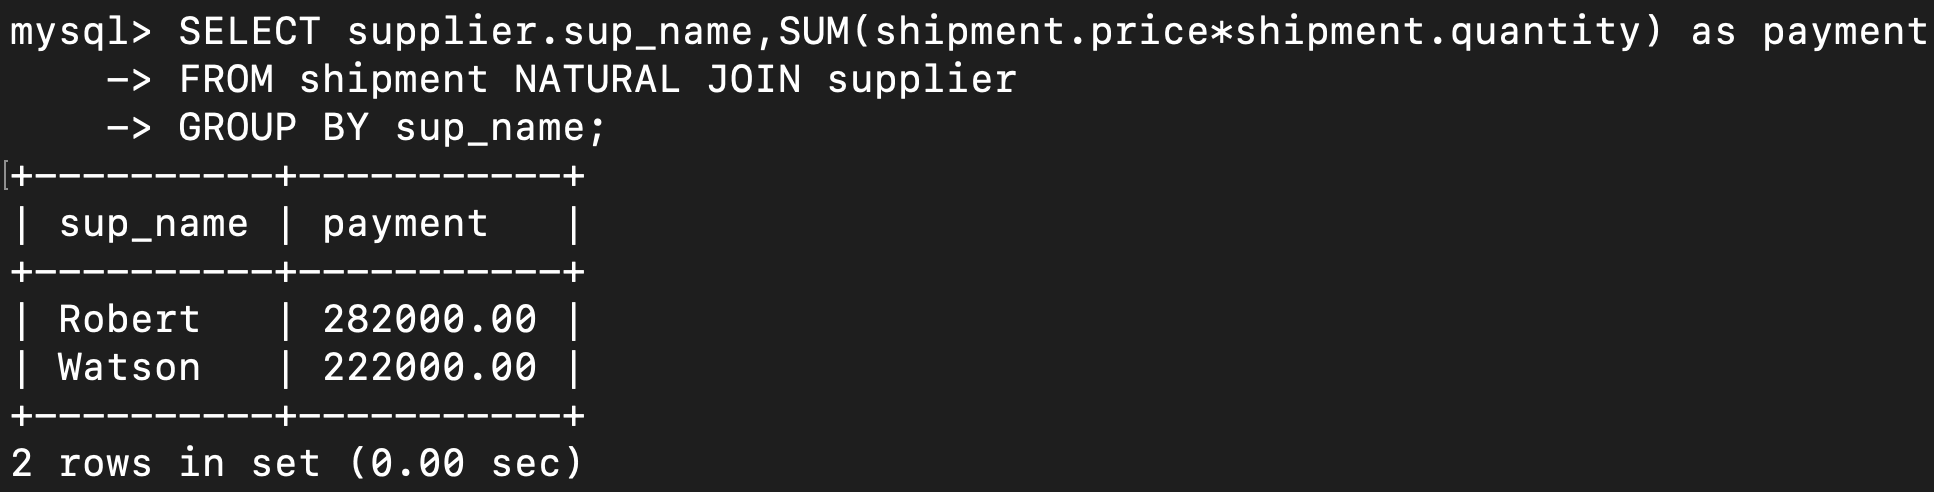
\includegraphics[scale=0.5]{screenshots/5b.png}
    \label{fig:my_label1}
\end{figure}

\subsection{Suppliers who have supplied all parts}

\subsubsection{Query}
\fbox{ \begin{minipage}{40em}
\inputminted{mysql}{src/question5c.sql}
\end{minipage}
}

\subsubsection{Result}
\begin{figure}[!hbt]
    \centering
    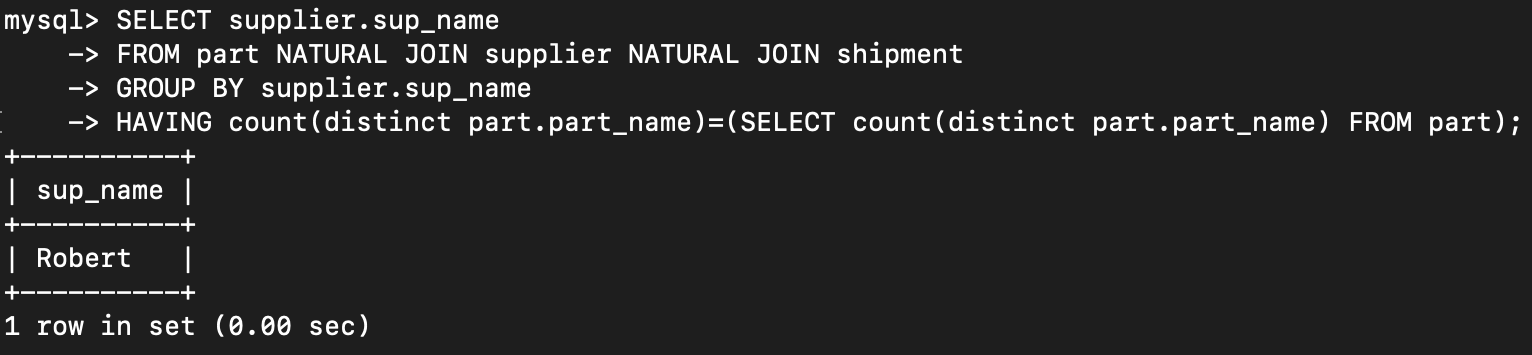
\includegraphics[scale=0.65]{screenshots/5c.png}
    \label{fig:my_label1}
\end{figure}
\newpage

\end{document}